\scanpage{67}
% block: title
\uline{Catégories tannakiennes définies par des cristaux}.

% block: crystals item 1
\handwritten{1.} Soit $k$ un corps de car. $p>0$, q\handwritten{u'}on regarde comme algèbre sur $\underline{Z}_p$, dont l'idéal maximal est muni de puissances divisées. Cela donne un \unsure{\deleted{e}s|\deleted{s}e}ens au site cristallin de $k$ (sur $\underline{Z}_p$, q\handwritten{u}alifié aussi de ``absolu''), et aux Modules loc. libres de type fini\inserted{(resp. de p\unsure{\deleted{t}r|r|t}ésentation finie)}\handwritten{\begin{tikzpicture}[x=1cm,y=1cm,baseline=-.1cm]\draw[thin] (0,.15).. controls (.05,-.1) and (-.2,-.1)..(-1,-.1)--(-2.1,-.1).. controls (-2.3,-.1) and (-2.35,-.2)..(-2.35,-.5);\end{tikzpicture}} sur ledit, qu'on appellera aussi cristaux en modules (localement libres\inserted{resp. de prés; finie}\handwritten{\begin{tikzpicture}[x=1cm,y=1cm,baseline=-.1cm]\draw[thin] (0,.15).. controls (.05,-.1) and (-.2,-.1)..(-1,-.1)--(-2.1,-.1).. controls (-2.3,-.1) and (-2.35,-.2)..(-2.35,-.5);\end{tikzpicture}}) sur $k$. Ces cristaux forment une $\otimes$-catégorie $\underline{Z}_p$-linéaire, \deleted{avec des $\operatorname{Hom}$ qui sont des modules de type fini sur $\underline{Z}_p$} On peut expliciter cette catégorie à l'aide d'un $p$-anneau $W$ de corps résiduel $k$, comme la catégorie des modules libres de type fini (resp. de type fini) $M$ sur $\unsure{\mathbb{W}|W}$, avec pour tout entier $n$ une connexion absolue sur $M_n=M/p^nM$ (relativement à 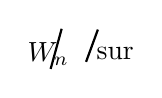
\begin{tikzpicture}[x=1cm,y=1cm,baseline=(w.base)]\node[inner sep=0pt] (w) at (0,0) {$W_n$};\node[inner sep=0pt] at (.85,0) {sur};\draw[thick] (.03,-.19)--(.17,.32);\draw[thick] (.48,-.1)--(.63,.31);\end{tikzpicture} $\underline{Z}/p^n\underline{Z}$), à courbure nulle, ces connexions se recollant pour $p$ variable. Lorsque $\deleted{p}\handwritten{k}$ est parfait, $W$ est l'anneau des vecteurs de Witt construit sur $k$, et dans la description précédente, on peut oublier les connexions: les catégories envisagées sont simplement la catégorie des modules libres de t.f (resp. des modules de t.f.) sur $W$. Si $K$ est le corps des fractions de $W$, la catégorie des \uline{isocristaux} \deleted{sur} (=cristaux à isogénie près) sur $k$ est équivalente à $\operatorname{Modf}(K)$. \deleted{C'est une catégorie tannakienne sur $\underline{Q}_p$}

% block: crystals item 2
\handwritten{2.} La catégorie des cristaux\unsure{\deleted{n}|n} sur $k$ dépend fonctoriellement de $k$, d'où pour tout cristal la possibilité de définir son transformé par le changement de base $\handwritten{\unsure{\sigma|\deleted{\illegible{1}}\sigma}}_k:x\handwritten{\mapsto}x^p:\ k\handwritten{\longrightarrow}k$, soit $M^{\handwritten{\unsure{\sigma|\sigma'}}}$. La donnée d'un $M$ avec un hèmomorphisme
\[
F_M:\ M^{\handwritten{\sigma}}\handwritten{\longrightarrow}M
\]
s'appelle un $F$\handwritten{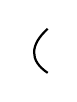
\begin{tikzpicture}[x=1cm,y=1cm,baseline=-.05cm]\draw[thick] (.12,.3).. controls (-.1,.1) and (-.12,-.1)..(.12,-.26);\end{tikzpicture}}-\uline{cristal sur} $k$. On notera que les $F$-cristaux forment une\inserted{$\otimes$-}\handwritten{\begin{tikzpicture}[x=1cm,y=1cm,baseline=-.1cm]\draw[thin] (0,.3).. controls (0,0) and (-.5,-.05)..(-.55,-.45);\end{tikzpicture}}catégorie\inserted{$\underline{Z}_p$-linéaire}\handwritten{\begin{tikzpicture}[x=1cm,y=1cm,baseline=-.1cm]\draw[thin] (0,.15).. controls (.05,-.1) and (-.2,-.1)..(-1,-.1)--(-2.1,-.1).. controls (-2.3,-.1) and (-2.35,-.2)..(-2.35,-.5);\end{tikzpicture}} dont les $\operatorname{Hom}$ sont des modules de type fini sur $\underline{Z}_p$ (attention, pas\inserted{\handwritten{des modules}}\handwritten{\begin{tikzpicture}[x=1cm,y=1cm,baseline=-.1cm]\draw[thin] (0,.15).. controls (.05,-.1) and (-.2,-.1)..(-1,-.1)--(-2.1,-.1).. controls (-2.3,-.1) and (-2.35,-.2)..(-2.35,-.5);\end{tikzpicture}} sur $W$, même si $k$ est parfait !). Ce n'\unsure{\deleted{t}e|\deleted{i}e|e}st pas une \deleted{\unsure{catégorie|ctatégorie}} catégorie tannakienne, même une fois tensorisée par $\underline{Q}_p$, car il manqu
% archive sheet number: 66
